\documentclass[12pt,a5]{scrartcl}
\usepackage[english]{babel}
\usepackage{natbib}
\usepackage{hyperref}
\usepackage[utf8x]{inputenc}
\usepackage{amsmath}
\usepackage{graphicx}
\graphicspath{{images/}}
\usepackage{parskip}
\usepackage{fancyhdr}
\usepackage{vmargin}
\setmarginsrb{3 cm}{2.5 cm}{3 cm}{2.5 cm}{1 cm}{1.5 cm}{1 cm}{1.5 cm}

\title{From Python to Guile Scheme}                                % Title
\author{}                               % Author
\date{}                                         % Date

\makeatletter
\let\thetitle\@title
\let\theauthor\@author
\let\thedate\@date
\makeatother

\pagestyle{fancy}
\fancyhf{}
\rhead{\theauthor}
\lhead{\thetitle}
\cfoot{\thepage}

\begin{document}

%%%%%%%%%%%%%%%%%%%%%%%%%%%%%%%%%%%%%%%%%%%%%%%%%%%%%%%%%%%%%%%%%%%%%%%%%%%%%%%%%%%%%%%%%

\begin{titlepage}
    \centering
    \vspace*{0.0 cm}
        \textsc{\LARGE Free Digital Version of}\\[0.5 cm]  % University Name
    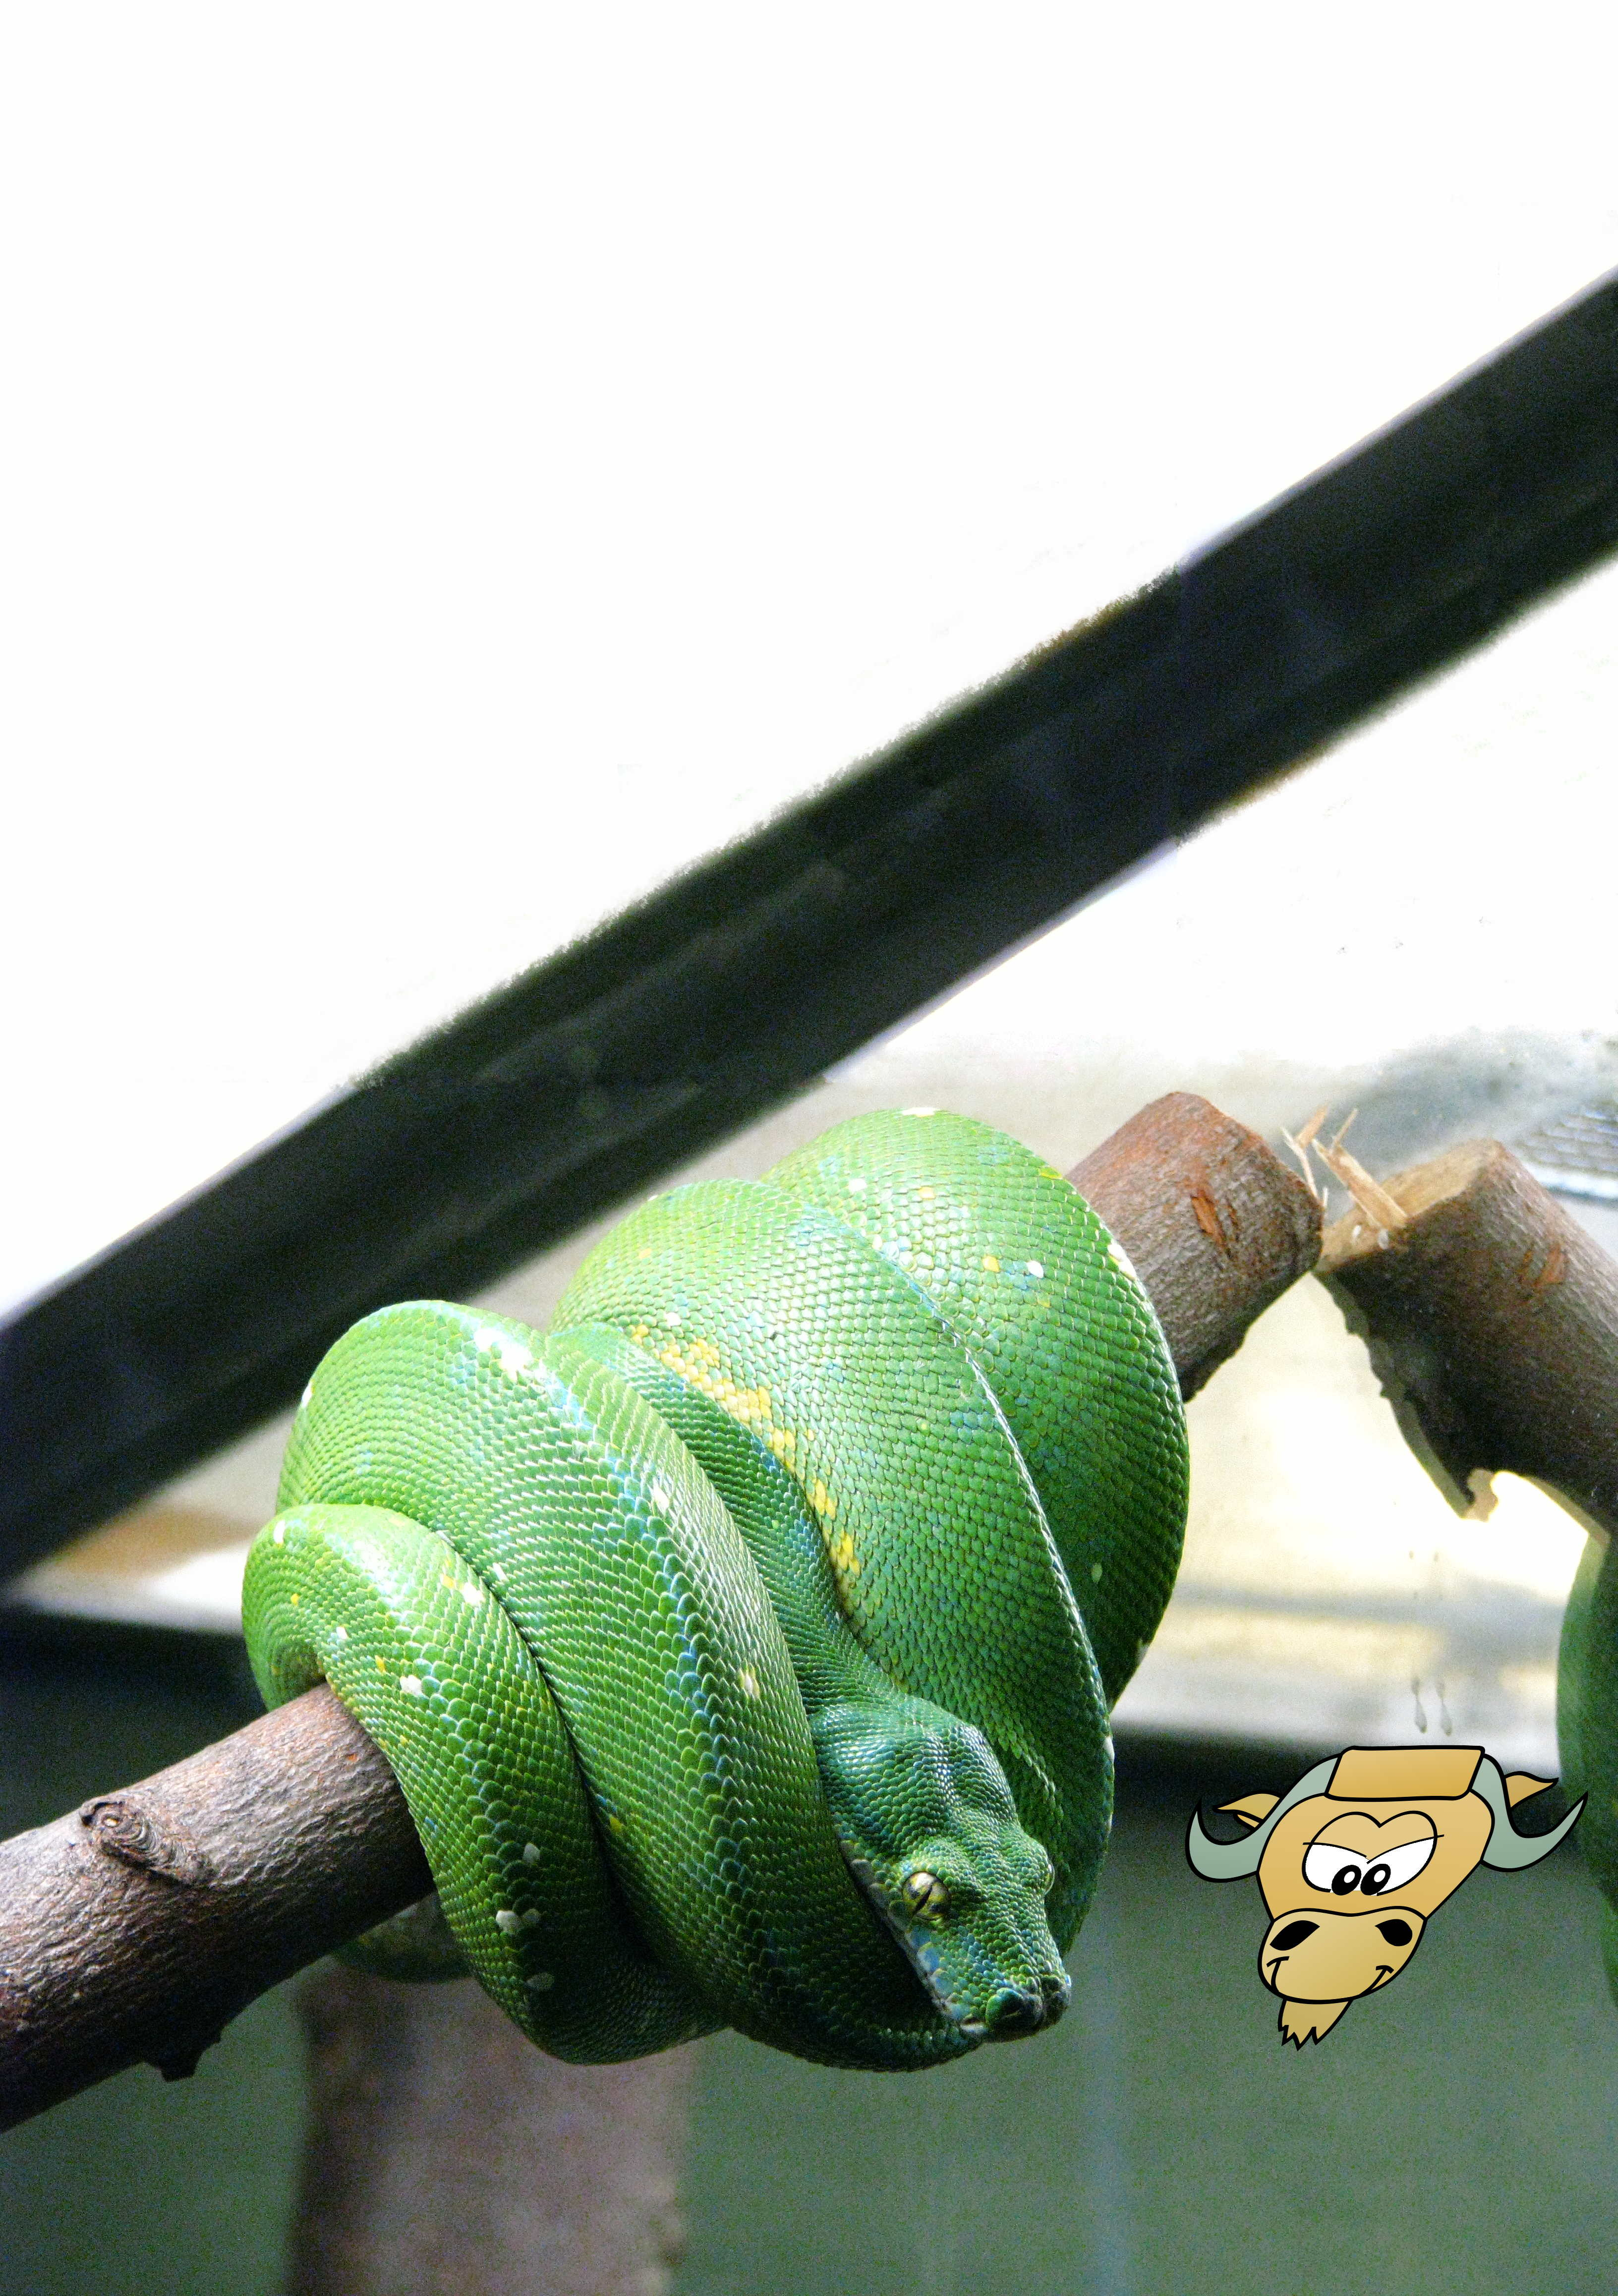
\includegraphics[height=0.5\textwidth]{green_tree_python-flickr-author-msvg-michael_gil-license-cc_by-4533044418_707b0029b2_o-and-guile-gnu-goatee-by-martin-grabmueller-license-gplv3-or-later-unified-resynth.jpg}\\[1.0 cm]  % University Logo
    \rule{\linewidth}{0.2 mm} \\[0.4 cm]
    { \huge \bfseries \thetitle}\\
    \centering \rule{\linewidth}{0.2 mm} \\[1.5 cm]
    \textsc{\Large If you enjoy this book,\\[0.3cm] please buy the ebook or print from\\[0.7 cm] \textbf{\href{http://draketo.de/py2guile}{http://draketo.de/py2guile}}}\\[0.5 cm]               % Course Code

    \textsc{\Large Buy free licensed creations,\\[0.5cm] so I can create more.}
    
    
\end{titlepage}

%%%%%%%%%%%%%%%%%%%%%%%%%%%%%%%%%%%%%%%%%%%%%%%%%%%%%%%%%%%%%%%%%%%%%%%%%%%%%%%%%%%%%%%%%


\end{document}